\documentclass[12pt,a4paper]{article}%
\usepackage[utf8]{inputenc}

%%%% pour ne pas compiler les images
\usepackage{graphicx}
%\usepackage[draft]{graphicx}

\usepackage{ulem}
\usepackage{amsmath}
\usepackage{amsfonts}
\usepackage{amssymb}
\usepackage[T1]{fontenc}%
\setcounter{MaxMatrixCols}{30}

\providecommand{\U}[1]{\protect\rule{.1in}{.1in}}
%EndMSIPreambleData
\usepackage{color}
\renewcommand{\@}{\textcolor{red}}
\newcommand{\ed}{\textsc{EcoDyco}}

\begin{document}


\thispagestyle{empty}

\date{}

\begin{center}
{\Huge {\ed} \\[0pt]}

{\Huge \textbf{User Manual} \\[0pt]}
\end{center}

\vskip 5.0em

\begin{figure}[h]
\centering 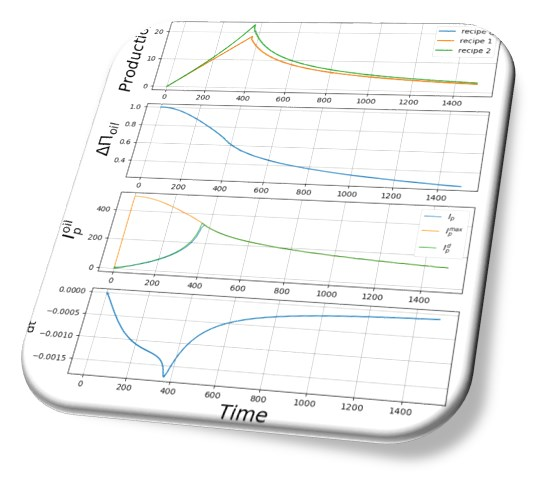
\includegraphics[width=1.0\textwidth]{figures/couverture.jpg}\end{figure}

\vskip 5em

\begin{center}
{\LARGE \textbf{Version 1.0} }
\end{center}

\normalfont


\vskip 1.5em


\vskip 10.0em

\newpage
\thispagestyle{empty}
\tableofcontents
\setcounter{page}{1}
\newpage

\section{\ed: An economic model in a finite physical world}

%Le modèle \ed\ a été conçu sur la base de cinq constats :
%
%\begin{enumerate}
%\item Si le monde physique est modifié par l'application des lois de
%l'économie, il n'en demeure pas moins que son évolution est gouverné pas des
%lois physiques.
%
%\item Le monde physique est fini, ceci est vrai pour toutes les ressources
%matérielles et pour les ressources énergétiques fossiles.
%
%\item Dans un monde fini, la définition d'une fonction de production doit prendre en compte l'état des ressources. La production est contingente de la ressource disponible.
%
%\item L'intensité de prélèvement d'une ressource est un facteur majeur
%agissant sur le devenir de cette dernière.
%
%\item Si l'économie n'est pas descriptible strictement par la thermodynamique,
%cette dernière peut lui fournir certaines catégories utiles, et, en
%particulier, la distinction entre \textit{quantité} et \textit{qualité},
%elles-mêmes reliées au caractère intensif ou extensif des variables.
%\end{enumerate}

The model \ed\ was designed on the basis of five findings:

\begin{enumerate}
	\item If the physical world is modified by the application of the laws of the economy
	of the economy, the fact remains that its evolution is governed by
	physical laws.
	
	\item The physical world is finite, this is true for all material resources
	resources and for fossil energy resources.
	
	\item In a finite world, the definition of a production function must take into account the state of the resources. Production is contingent on the available resource.
	
	\item The intensity of withdrawal from a resource is a major factor
	on the fate of the resource.
	
	\item If the economy is not strictly describable by thermodynamics,
	thermodynamics can provide it with some useful categories, and in particular the
	In particular, the distinction between \textit{quantity} and \textit{quality},
	themselves linked to the intensive or extensive character of the variables.
\end{enumerate}


\noindent These findings form the basis for the structure and operation of the model \ed.

\begin{enumerate}
	\item The descriptions of the physical and economic spheres of the model
	are disjointed. They communicate through specific variables and parameters. 
	
	\item Each resource is described in its own sheet. The collection of sheets thus obtained is the physical sphere. Each sheet quantifies the usable fraction and the used fraction of the
	Each sheet quantifies the usable fraction and the used fraction of the resource, which we will call waste. The used fraction can only be used again
	used again only after recycling.
	
	\item It is defined a production query function called "demand", which
	replaces, for the physical dimension, the production function. The structure and the parameterisation 
	The structure and parameterisation of the production function are fixed by the specific choices
	The structure and parameterisation of the production function are fixed by specific choices made in the economic area of the model.
	
	\item It is defined an intensity of operation of the economy which governs
	the whole of the physical sheets.
	
	\item The quantities of resources are also associated with qualities, which, like the first and second principles, are
	the image of the first and second principles of thermodynamics, define,
	the difference in quality of a resource and its state of transformation, towards a
	transformation, towards a product or towards a waste.
\end{enumerate}


\section{General structure of \ed}

The model is structured in sheets of stock type and flow type,
linked to the economic module. Its overall architecture is as follows:


\begin{figure}[h]
\centering \includegraphics[width=1.0\textwidth]{figures/Archiglobale.jpg}\end{figure}

\subsection{Structure of a Stock sheet}

Stock sheets are intended for most resources, mineral, fossil or not, whose quantity on the planet is finite and of variable dispersion.

\begin{figure}[h]
\centering
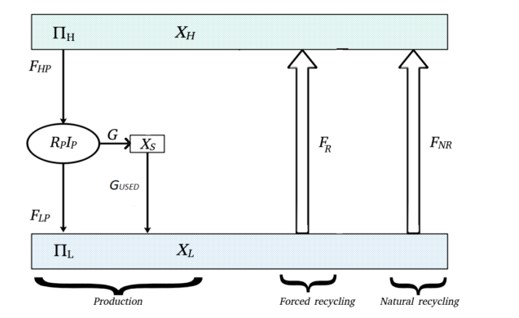
\includegraphics[width=1.0\textwidth]{figures/FeuilleStock.jpg}\end{figure}

On a typical sheet of paper, there is a high zone containing the resource in quantity $X_{H}$ and quality $\Pi_{H}$ and a zone of used resource in quantity $X_{L}$ and quality $\Pi_{L}$. The resource flows of $F_{HP}$ and the waste flows $F_{LP}$ constitute, together with the production flow $G$, the whole of the resource flows in its implementation for production.
The quantity of resource used in excess constitutes a stock $X_{S}$. Recycling can be natural $F_{NR}$, or forced, $F_{R},$ according to specific laws. We call the difference of potentials the quantity $\Delta \Pi=\Pi_{H}-\Pi_{L}$.



\subsubsection{Stock sheet parameters}

A stock sheet is initially defined by the set of limited parameters listed below, values are given as an example.

\begin{itemize}
\item Son type: \textit{type : stock}

\item Son nom: \textit{name : cuivre}

\item Sa quantité totale: \textit{total stock : 500000}

\item Son niveau de ressource initial: \textit{Xh\_init : 500000}

\item Son niveau de déchet initial: \textit{Xl\_init : 0}

\item Sa résistance de dissipation de production~:\textit{\ Rp0 : 0.003}

\item Le niveau de capital initial associé a l'appareil de
production\textit{\ K0 : 1}

\item Ratio énergétique de recyclage (1 unité d'énergie pour recycler 1 unité
de la ressource)~:\textit{\ recyclingEnergyFlux : 1}

\item Utilisable comme énergie (cas du pétrole)~:\textit{\ isEnergy : False}

\item Taux de recyclage naturel (r=0~: pas de recyclage)~:\textit{\ r : 0}

\item Temps caractéristique~:\textit{\ to : 9}
\end{itemize}

The description and use of these parameters is described in detail in the
in the annexes to this document. However, special attention is paid to
particular attention is paid to $R_{P}$.

\subsubsection{Résistance de dissipation: R$_{P}$}
The dissipation resistance is a term that intervenes, via the production intensity, in the form $R_{P}I^{2}$. This term indicates the fraction of the resource that is not used for the production of consumer goods, even though the resource has been taken from the planet. $R_{P}$ leads to a limitation of the capacity of a production tool that cannot operate at high intensity. An efficient production tool is associated with a low value for $R_{P}$. As a main parameter that drive the production tool $R_{P}$ is therefore directly linked to capital. It follows that $R_{P}$ naturally increases over time under the effect of the degradation of the capital. For the same reason, investment efforts lead to reduce $R_{P}$. The same is true of technical progress which results in a sudden drop in $R_{P}$ under the effect of the implementation of this new method. Finally, with constant technical progress, the multiplication of production site corresponds to the setting in parallel of several resistances, which leads to a reduction of the global resistance by the same factor, thus allowing work to be carried out at a higher intensity since it is spread over the production sites. If a high value of $R_{P}$ reflects a production tool that is not compatible with in a production-intensive economy, inversely, it is clear that a low value of $R_{P}$ is not necessarily an enviable situation from an ecological point of view, in the sense that the very large capacity of the production tool is also
leads to increase massively the resource extraction. The accelerated scarcity of the resource of this sheet then leads to a pinch of production.

\noindent Four main effects can be attributed to the presence of $R_{P}$:

\begin{enumerate}
\item Dégradation du capital qui se traduit à une augmentation de $R_{P}$
avec les conséquences qui s'en suivent sur la qualité d'exploitation de la ressource.

\item Effet de l'innovation qui se traduit à une baisse de $R_{P}$ avec
les conséquences qui s'en suivent sur la quantité de prélèvement accrue de
la ressource.

\item Augmentation de la capacité de production, à progrès constant,
qui se traduit à une baisse de $R_{P}$ global avec les conséquences qui
s'en suivent sur la quantité de prélèvement accrue de la ressource.

\item Effet de l'investissement qui se traduit à une baisse de $R_{P}$
avec les conséquences qui s'en suivent sur la quantité de prélèvement
accrue de la ressource.
\end{enumerate}

It should also be noted that whatever the value of $R_{P}$, a decrease in production yields is observed for production intensities above a certain threshold. In this sense, $R_{P}$ contributes to the Ricardian character of the appearance of diminishing returns.  It is important to note that the limitation of yields also originates in the mechanism of resource scarcity, which is highlighted by the decrease in the difference in potential $R_{P}$.\footnote{
	The question of the capacity for indefinite growth thus finds its main ingredients here, namely:
	\begin{enumerate}
		\item The decline in yields as a function of the intensity of harvesting, beyond a certain threshold.
		\item The drop in production due to the unavailability of the resource (pinch) is present at the heart of the mechanism of each of the sheets. It thus appears that the flow of extraction of the resources depends at the same time on the capacities of production (via $R_{P}$) installed and on the difference of potential $\Delta\Pi$.
	\end{enumerate}}

\subsection{Structure d'un feuillet flux}

Les feuilles de type flux sont destinées aux ressources qui sont disponible
sur la planète sous la forme d'un flux. La plus usuelle étant
naturellement l'énergie solaire.

\begin{figure}[h]
\centering
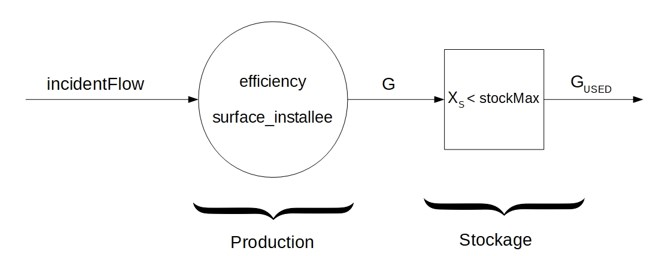
\includegraphics[width=1.0\textwidth]{figures/FeuilleFlux.jpg}\end{figure}

\subsubsection{Paramètre de feuillet flux}

Un feuillet flux est défini initialement par le jeu des paramètres limités
dont la liste est donnée ci-dessous (Les valeurs sont données à titre d'exemple):

\begin{itemize}
\item Son type~:\textit{\ type : flow}

\item Son nom \textit{name : energie solaire}

\item Le flux incident~: \textit{incidentFlow : 1e10}

\item L'efficacité de conversion~: \textit{eff\_init : 0.15}

\item La surface installée \textit{surface\_installee : 1e-9}

\item Utilisable comme énergie: \textit{isEnergy : True }

\item Capacité maximale de stockage~: \textit{stockMax\_init : 50}
\end{itemize}

\subsection{Structure du noyau physique}

Le noyau physique est le lieu de la réalisation des biens manufacturés. Le
schéma de principe du fonctionnement de cette zone est donné dans la figure ci-dessous.

\begin{figure}[h]
\centering 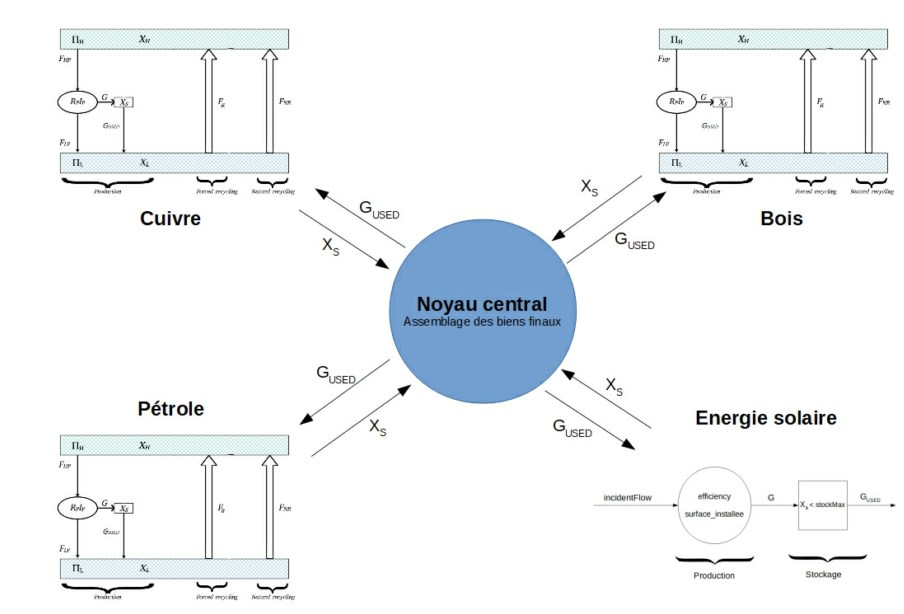
\includegraphics[width=1.0\textwidth]{figures/NoyauCentral.jpg}\end{figure}

Les "recettes" de fabrication des biens manufacturés sont indiquées dans la
feuille \textit{world.txt}. Le programme principal effectue automatiquement la
réalisation en respect de ces "`recettes"'.

\subsection{Structure de la zone économique}

La zone économique est le lieu ou est codé le modèle économique sur lequel
se fonde la simulation. Afin d'illustrer ce point, deux exemples de
modèles sont données~:

\begin{enumerate}
\item Goodwin

\item Sollow
\end{enumerate}

L'utilisateur avancé peut construire son propre modèle en suivant la
structure générale d'une feuille économique.~(voir Annexe A)

\section{Simuler avec \ed}

\subsection{Liste des fichiers}

Vous devez avoir dans un dossier:

\begin{itemize}
\item les scripts python :

\begin{itemize}
\item le fichier \textbf{PhysicalWorld.py}

\item un fichier décrivant votre sphère économique. Dans
ce manuel nous nous appuierons sur le modèle de Goodwin, décrit ans le fichier \textbf{Goodwin.py}.

\item le fichier \textbf{main.py}
\end{itemize}
\end{itemize}

\begin{itemize}
\item autant de fichiers de paramétrage que nécessaire. Au moins un feuillet doit être utilisé.

\begin{itemize}
\item \textbf{world.txt} (indispensable)

\item \textbf{oil.txt} si vous avez une feuille pétrole

\item \textbf{copper.txt} si vous avez une feuille cuivre

\end{itemize}
\end{itemize}

Il suffit d'exécuter le fichier main.py.\newline On modifie dans main.py le
pas de temps \textit{deltat}, et l'étendue temporelle de la simulation
\textit{tmax}.

\subsection{Paramétrage de la sphère physique}

Pour modifier les paramètres physiques (paramètres des cellules, et
paramètres globaux de la sphère physique), il faut modifier les
fichiers .txt correspondant.

\subsubsection{Ajout d'une cellule}

Paramétrage de la nouvelle cellule:

\begin{enumerate}
\item pour créer une cellule stock, prendre le template StockCell.txt, rentrer
les paramètres souhaités, et enregistrer sous le nom de la ressource (ex~: cuivre.txt)

\item pour créer une cellule flux, faire de même avec le template FlowCell.txt

\item ensuite, ajouter dans world.txt votre nouvelle cellule dans le tableau cells.

\item enfin, rajouter la colonne correspondante a recipeMatrix dans world.txt
\end{enumerate}

\subsubsection{Retrait d'une cellule}

\begin{enumerate}
\item Supprimer la cellule dans le tableau cells de world.txt

\item Supprimer la colonne correspondante de recipeMatrix dans world.txt
\end{enumerate}

\subsubsection{Modification des paramètres et valeurs initiales des
variables de la sphère physique}

\begin{itemize}
\item Les paramètres globaux et valeurs initiales des variables globales
de la sphère physique sont stockés dans les fichiers world.txt.

\item Les paramètres et valeurs initiales des variables des feuilles sont
stockés dans les fichiers \textit{nom\_de\_la\_feuille.txt}.

\item Ne pas oublier d'enregistrer le fichier \textit{.txt} apres modification d'une
valeur.\footnote{Attention, la lecture des paramètres dans les fichiers est
{peu robuste}. Il faut veiller a respecter l'espacement, ne pas rajouter un
saut de ligne a la fin, etc. En particulier, les chaînes de caractere du
tableau cell (par exemple ``~copper.txt~'') servent ensuite a rediriger vers le
fichier ``~copper.txt~'' pour l'initialisation de la feuille cuivre. Le nom du
fichier contenant les paramètres de la feuille doit donc etre la même chaîne
de caractere que celle qui apparaît dans cell.}

\item Le message \texttt{``~world successfully created~''} s'affiche dans la console
lorsque le modèle a été initialisé.
\end{itemize}

\subsection{Paramétrage de la zone économique: exemple Goodwin}

\begin{figure}[h]
\centering
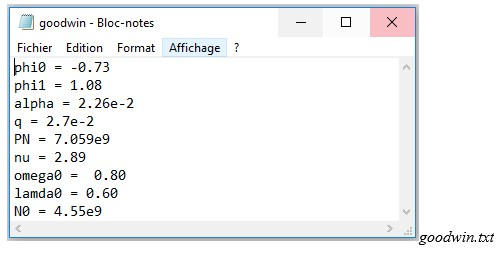
\includegraphics[width=1.0\textwidth]{figures/Goodwin-txt.jpg}\end{figure}

\begin{itemize}
\item $phi0$ et $phi1$ sont les paramètres de la courbe de Philipps

\item $alpha$ est le taux de croissance de la productivité du travail

\item $q$ est le taux de croissance de la population

\item $P_{N}$ est la valeur maximale de la population (le taux de croissance
réel de la population N est $q\ast (1-N/P_{N}))$

\item $nu$ est la productivité du capital

\item $omega0$, $lambda0$ et $N_{0}$ sont les valeurs initiales du wageshare,
employment rate et de la population
\end{itemize}

\newpage

\section{Etude de cas élémentaire}

\subsection{Paramétrisation}

On se propose d'illustrer le fonctionnement de \ed\ par une étude de cas
basée sur 

\begin{itemize}
\item 4 ressources : cuivre, bois, pétrole, solaire

\item  3 recettes: 

\begin{itemize}
\item 1 cuivre + 2 énergie => bien 0

\item 1 cuivre + 2 bois + 3 énergie => bien 1

\item 1 énergie => bien 3 (recyclage cuivre)
\end{itemize}

\item 1 Mix énergétique cible : 90\% solaire, 10\% pétrole
\end{itemize}

\begin{figure}[h]
\centering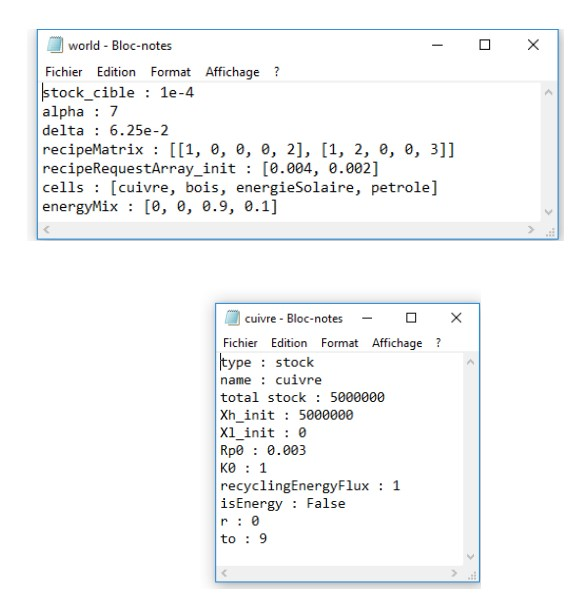
\includegraphics[width=0.7\textwidth]{figures/Parametrisation.jpg}
\end{figure}


Dans le fichier principal \textit{main.py}, on effectue 

\begin{enumerate}
\item le choix du fichier \textit{Solow.py} comme modèle économique

\item paramétré par le fichier \textit{solow.txt} 

\item le choix du pas de temps et de la durée de la simulation
\end{enumerate}

\begin{figure}[h]
\centering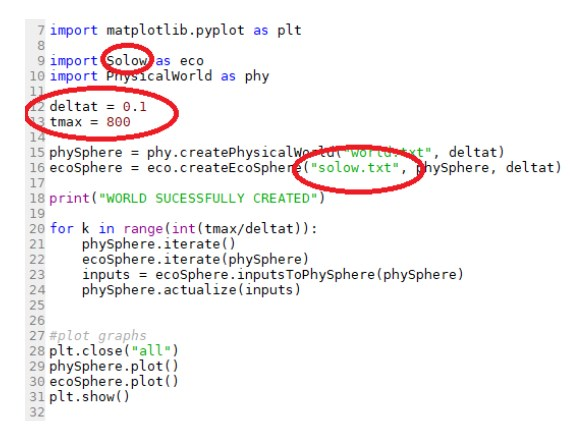
\includegraphics[width=0.8\textwidth]{figures/Parametrisation2.jpg}
\end{figure}


Dans le fichier du modèle économique on spécifie ses paramètres. (ici \textit{Solow.txt})

\begin{figure}[h]
\centering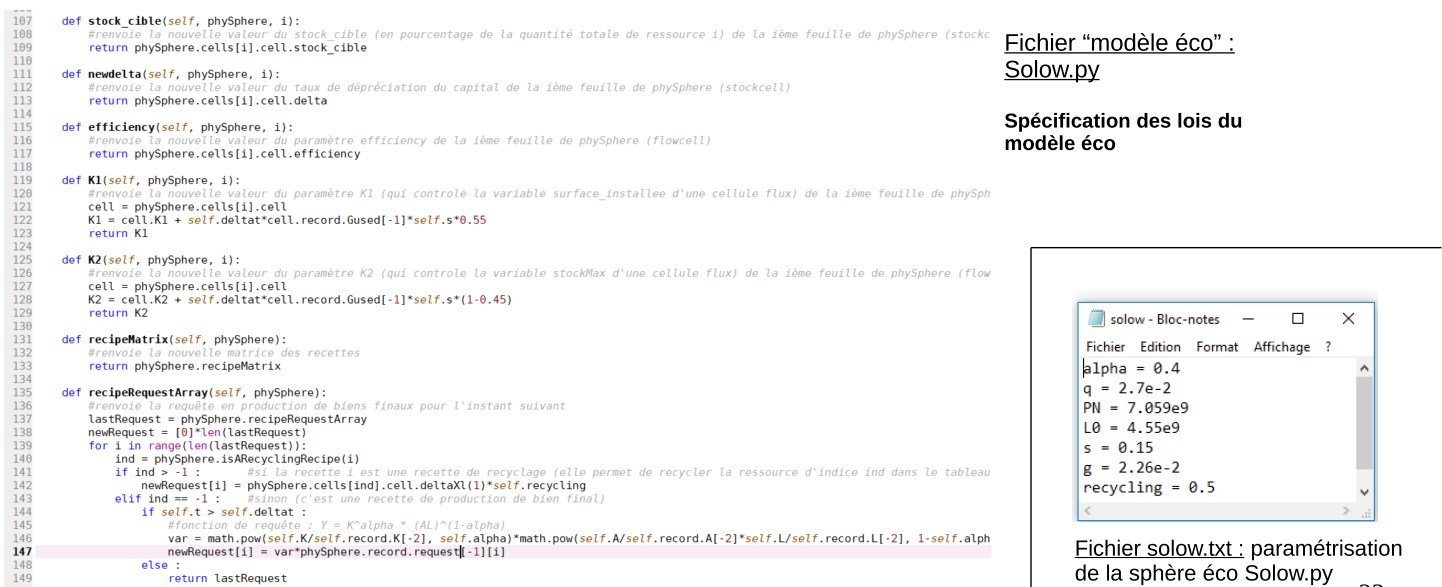
\includegraphics[width=0.95\textwidth]{figures/Parametrisation3.jpg}
\end{figure}

\subsection{Résultat}

Le lancement de la simulation via le module \textit{main.py} conduit au résultat
suivant pour la production et l'énergie:

\begin{figure}[h]
\centering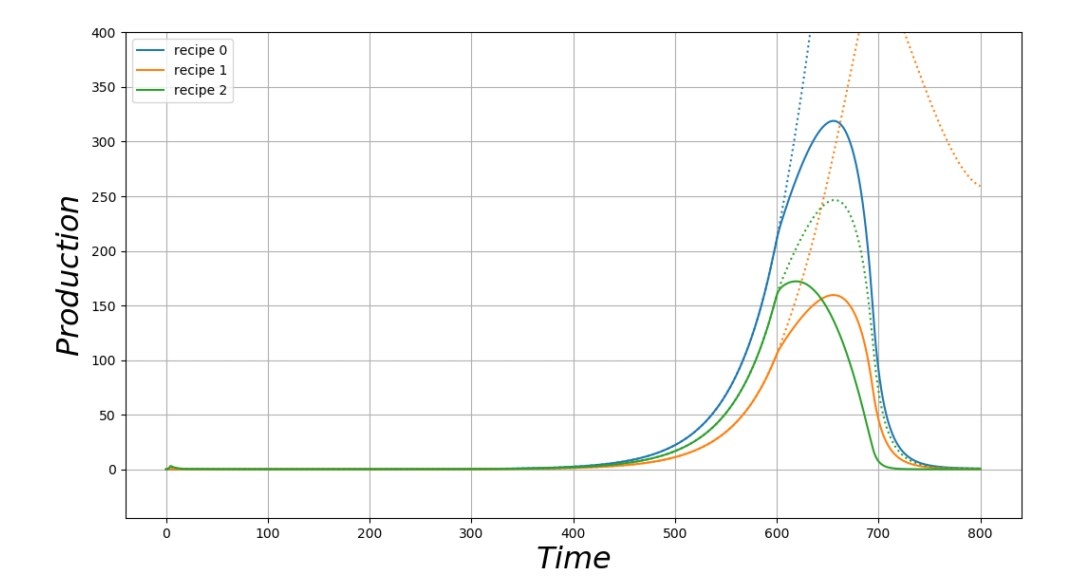
\includegraphics[width=0.7\textwidth]{figures/ResultatSimul.jpg}
\end{figure}

\begin{figure}[h]
\centering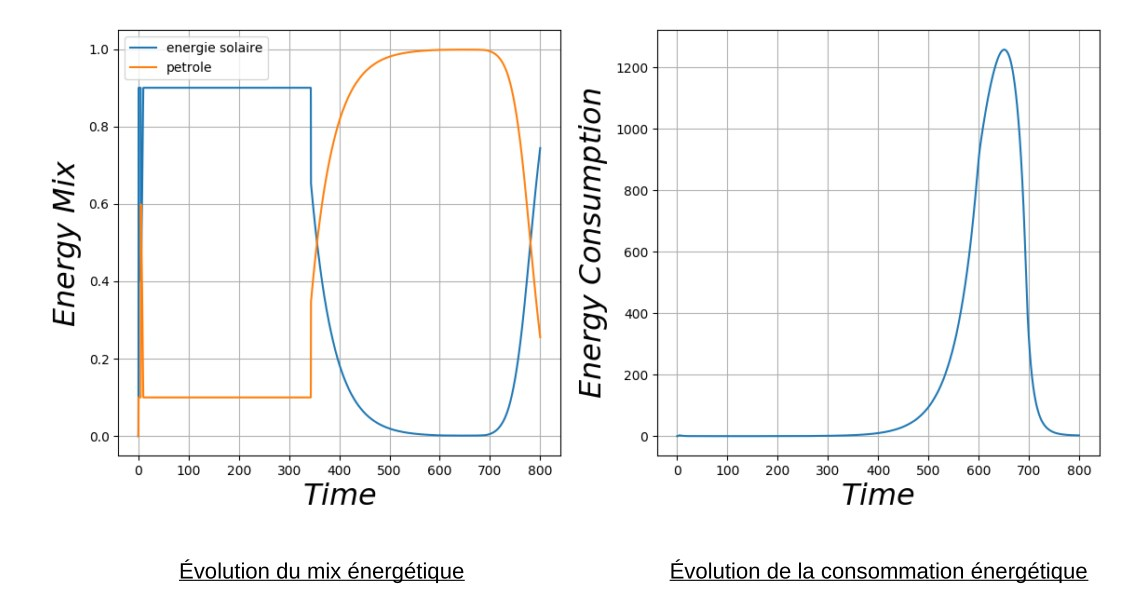
\includegraphics[width=0.7\textwidth]{figures/ResultatSimulE.jpg}
\end{figure}

Toutes les informations relatives à chacun des feuillets étant
enregistrées, il est possible de suivre les paramètres à volonté, par
exemple ici pour le pétrole:

\begin{figure}[h]
\centering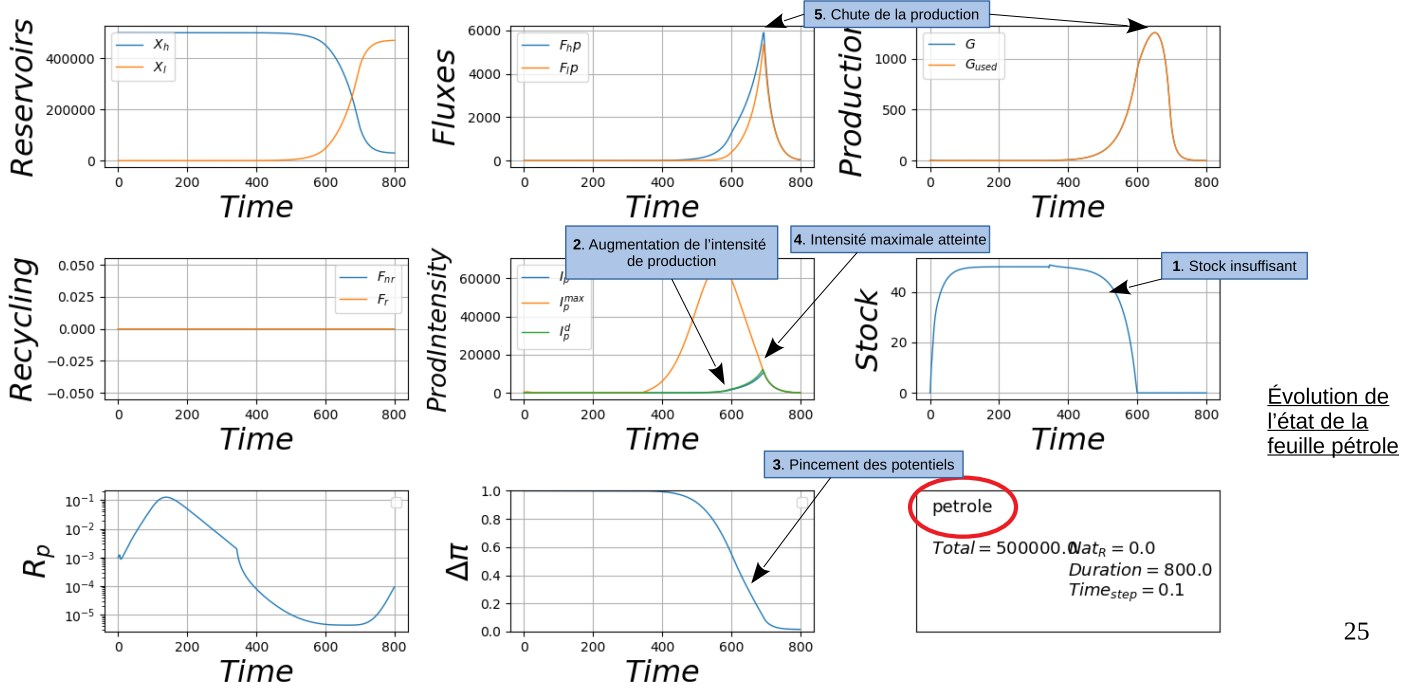
\includegraphics[width=0.7\textwidth]{figures/ResultatSimulPet.jpg}
\end{figure}

\newpage

\section{Annexe A: Comment utiliser un autre modèle économique~?}

\subsection{Utiliser un autre modèle économique parmi la bibliothèque
de modèles disponible}

Si l'on souhaite utiliser un modèle économique différent pour la
sphère économique, parmi les modèles disponibles, il faut effectuer
les modifications suivantes dans le fichier main.py

\begin{itemize}
\item Ligne 9~: Spécifier le nom du fichier .py décrivant la sphère éco
(ici Goodwin.py)

\item Ligne 17-18~: créer une instance de la sphère éco avec un appel de
la fonction eco.createEcosphère() - vérifier que les arguments pris par
cette fonction correspondent bien aux arguments demandés par la fonction
createEcoSphere de votre fichier EcoModel.py (ici Goodwin.py)

\item Ligne 36: De même, vérifier les arguments pris par la fonction ecoSphere.inv()

\item Ligne 40: De même, vérifier les arguments pris par la fonction ecoSphere.iterate()

\item Ligne 42: De même, vérifier les arguments pris par la fonction ecoSphere.newProdRequest()
\end{itemize}

\begin{figure}[h]
\centering
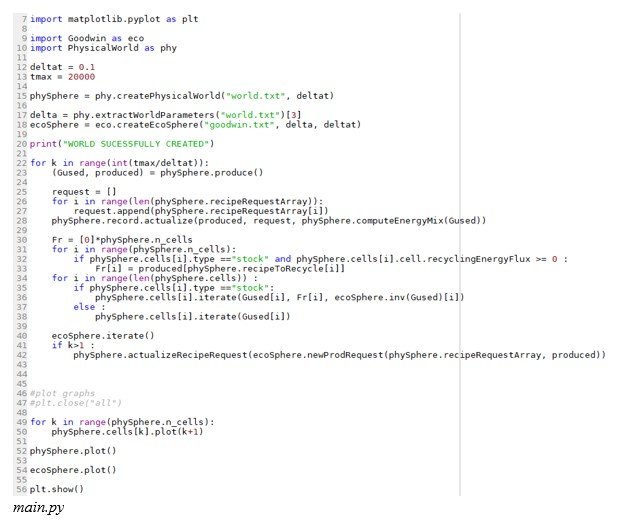
\includegraphics[width=1.0\textwidth]{figures/Main-py.jpg}\end{figure}

\subsection{Créer un nouveau modeles éco}

Il est possible d'insérer n'importe quel modèles économique au programme
DyCoEco. Si vous souhaitez en écrire un vous même pour l'ajouter a la
bibliothèque des modèles disponibles, vous devez respecter la
structure suivante dans votre script~:

Le fichier .py doit contenir :

\begin{itemize}
\item une fonction createEcoSphere
\end{itemize}

\begin{itemize}
\item une classe EcoSphere contenant :

\begin{itemize}
\item un constructeur \_\_init\_\_

\item une fonction iterate

\item une fonction inv

\item une fonction newProdRequest

\item une fonction plot
\end{itemize}
\end{itemize}

Un exemple de modèle économique (trivial) respectant cette structure est
donné ci-dessous (ecoVide.py).\newline Le rôle des fonctions citées ci-dessus
est également détaillé

\begin{figure}[h]
\centering
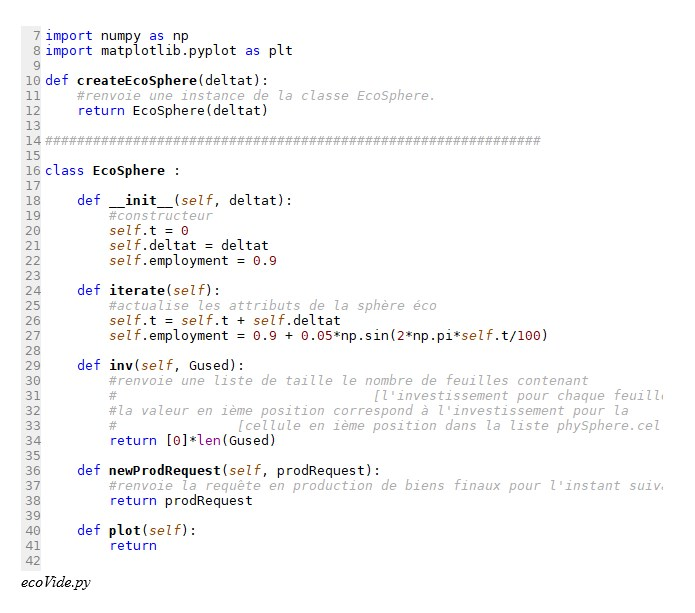
\includegraphics[width=1.0\textwidth]{figures/EcoVide-py.jpg}\end{figure}

\section{Annexe B: Equations gouvernants une feuille stock}

\subsection{Architecture générale}

Les ressources de type "~stock~" sont supposés être en quantité globale
constante. Une unité de ressource "~stock~" peut se trouver dans trois états différents.

Elle peut etre "\textit{disponible}~", c'est à dire pouvant être extraite
par l'appareil de production en vue d'une transformation ultérieure
(ressources valorisables). Elle peut également avoir déjà été extraite, et
être \textit{en attente} de transformation en bien final. Enfin, elle peut
etre \textit{usagée}, c'est à dire que la sphère économique est
incapable de la valoriser.

On définit trois réservoirs contenant les ressources dans chacun de ces trois
états : un \textit{réservoir haut} pour la fraction disponible de la
ressource, un \textit{stock} pour la fraction de la ressource en attente de
transformation ultérieure, et un \textit{réservoir bas} pour la fraction
usagée de la ressource.

On note $X_{H},X_{S}$ et $X_{L}$ les quantités correspondantes, et $X_{T}$ la
quantité totale de ressource.

Ainsi, on a a chaque instant :%

\[
X_{H}+X_{S}+X_{L}=X_{T}%
\]


Ensuite, on comptabilise strictement les mouvements entre ces trois réservoirs.

L'extraction de la ressource est le processus permettant de convertir une
unité de ressource "~disponible" en une unité de ressource "~en attente~". Ce
processus n'a le plus souvent pas une efficacité de 100\%: une fraction des
ressources disponibles extraites est immédiatement transformée en déchets. Ce
processus est analogue à la production de travail par un moteur thermique
: on produit, a partir de la différence de température entre deux thermostats,
une certaine quantité de travail utile W, tandis qu'une part de l'énergie
provenant de la source chaude $Q_{C}$ est dissipée sous forme de chaleur
$Q_{F}$.

\begin{figure}[h]
\centering
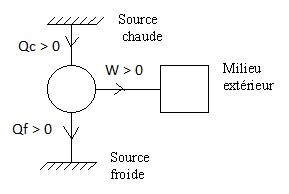
\includegraphics[width=0.6\textwidth]{figures/Carnot.jpg}\end{figure}

Ici, la source chaude devient le réservoir de ressource "~disponible~", la
source froide le réservoir de ressource "~usagée~", et le travail produit est stocké.

On note $F_{HP}$ le flux provenant du réservoir haut, $F_{LP}$ le flux en
direction du réservoir bas, et $G$ le flux de ressources en direction du
stock. Ainsi,%

\[
G=F_{HP}-F_{LP}%
\]


Les ressources dans le stock $X_{S}$ sont ensuite transformées en bien final.
Apres utilisation, la ressource devient déchet. On note $G_{USED}$ ce flux
entre le stock et le réservoir bas.

L'ensemble de ces flux définit la zone de production. Une unité de ressource
usagée peut parfois etre recyclée. Ce recyclage peut etre naturel, ou la
conséquence d'une activité humaine. On note $F_{NR}$ le flux de recyclage
naturel, et $F_{R}$ le flux de recyclage humain.

\subsection{Zone de production}

Au fur et à mesure que l'on exploite la ressource disponible, sa qualité
diminue, car on exploite la ressource de bonne qualité en premier. Or, la
qualité de la ressource a un impact sur l'effort a fournir pour l'extraire.
Par exemple, pour une ressource minière, il faut fournir un effort plus
important (\textit{l'intensité de production})\textit{\ }apres trois années
d'exploitation de la mine qu'au début de l'exploitation pour en extraire le
même flux. En effet, la qualité de la ressource (sa concentration notamment)
s'est dégradée. La notion de qualité est donc essentielle dans le processus
d'extraction. La thermodynamique établit bien cette distinction entre quantité
et qualité. On introduit donc ici une notion de thermodynamique, le
\textit{potentiel. }C'est une variable intensive. Les ressources dans le
réservoir haut sont a un certain niveau de potentiel, $\Pi_{H}$. $\Pi_{H}$
diminue au fur et a mesure de l'extraction de la ressource du stock haut.
$\Pi_{H}$ est donc une fonction croissante de $X_{H}$.

On a~:%
\[
F_{HP}=\Pi_{H}I_{P}%
\]
\ \ \ \ \ \ \ \ \ \ \ \ \ \ \ \ \ \ \ \ \ \ \ \ \ \ \ \ \ \ \ \ \ \ \ \ \ \ \ \ \
\[
\Pi_{H}=f_{1}(X_{H})
\]
\ \ \ \ \ \ \ \ \ \ \ \ \ \ \ \ \ \ \ \ 

Les déchets dans le réservoir bas sont une pollution, qui a une rétroaction
négative sur la production. Cette rétroaction se manifeste par l'augmentation
du potentiel du réservoir bas, $\Pi_{L}$.

On a~:\ \ \ \ \ \ \ \ \ \ \ \ \ \ \ \ \ \ \
\begin{align*}
\ F_{LP}  &  =\Pi_{L}I_{P}\\
\Pi_{L}  &  =f_{2}(X_{L})
\end{align*}


Le choix des fonctions $f_{1}$et $f_{2}$est important si l'on souhaite obtenir
des résultats quantitatifs avec le modèles. Si l'on ne souhaite que des
résultats qualitatifs, on peut se contenter de décrire la forme que devraient
avoir ces fonctions (croissante ou décroissante, concave ou convexe,
etc...)$_{.}$ Dans la suite, on prendra pour $f_{1}$ une fonction croissante
et convexe, telle que $f_{1}(X_{H}=0)=0,5$ et $f_{1}(X_{H}=X_{T})=1$. On
prendra pour $f_{2}$ une fonction croissante et concave, telle que
$f_{1}(X_{L}=0)=0etf_{1}(X_{L}=X_{T})=0,5$.

\begin{figure}[h]
\centering
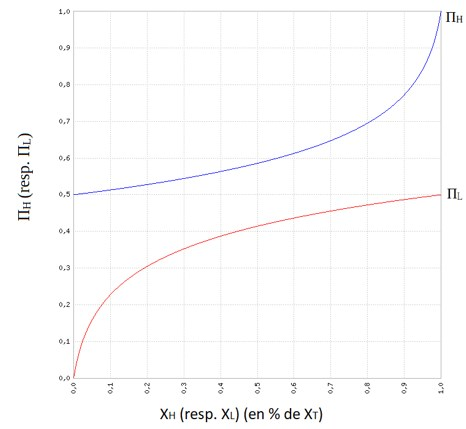
\includegraphics[width=1.0\textwidth]{figures/Potentiels.jpg}\end{figure}

Lorsque toute la ressource est dans le réservoir haut, $\Pi_{H}=1$ et $\Pi
_{L}=0$. La \textit{différence de potentiel }$\Delta\Pi$ est maximale. Lorsque
toute la ressource est dans le réservoir bas, $\Pi_{H}=\Pi_{L}=0,5$. La
différence de potentiel est nulle, et la production est impossible. L'activité
économique sans recyclage entraîne le passage de ressources entre le réservoir
haut et le réservoir bas, donc une diminution de $\Delta\Pi$. Autrement dit,
l'activité économique sans recyclage entraîne une diminution de la capacité
ultérieure à produire.

Finalement, on a introduit des variables extensives pour décrire la quantité
$(X_{H},X_{L},X_{S},X_{T})$, et des variables intensives pour décrire la
qualité de la ressource $(\Pi_{H},\Pi_{L})$

Le temps joue un rôle dans le processus d'extraction de la ressource. Plus
précisément, produire a une \textit{intensité }tres élevée n'est pas
équivalent a produire a faible \textit{intensité.} A faible intensité, le
rendement du processus est meilleur, mais le flux produit $G$ est moins
important. A intensité élevée, $G$ est plus élevé mais le rendement est dégradé.

On introduit donc une \textit{résistance} $R_{P}$. On a alors un terme de
friction $R_{P}I_{P}^{2}$, et $F_{LP}$
devient~:$\ \ \ \ \ \ \ \ \ \ \ \ \ \ \ \ $%
\[
F_{LP}=\Pi_{L}I_{P}+R_{P}I_{P}^{2}%
\]


En résumé, les équations décrivant l'extraction sont~:%
\begin{align*}
F_{HP}  &  =\Pi_{H}I_{P}\\
F_{LP}  &  =\Pi_{L}I_{P}+R_{P}I_{P}^{2}\\
G  &  =F_{HP}-F_{LP}=\Delta\Pi I_{P}+R_{P}I_{P}^{2}%
\end{align*}
\ \ \ \ \ \ \ \ 

Le flux extrait G est donc fonction de la différence de potentiels, de
l'intensité de production, et de la résistance. Supposons $\Delta\Pi$ et
$R_{P}$ fixés. G est alors une fonction parabolique de $I_{P}$.

\begin{figure}[h]
\centering
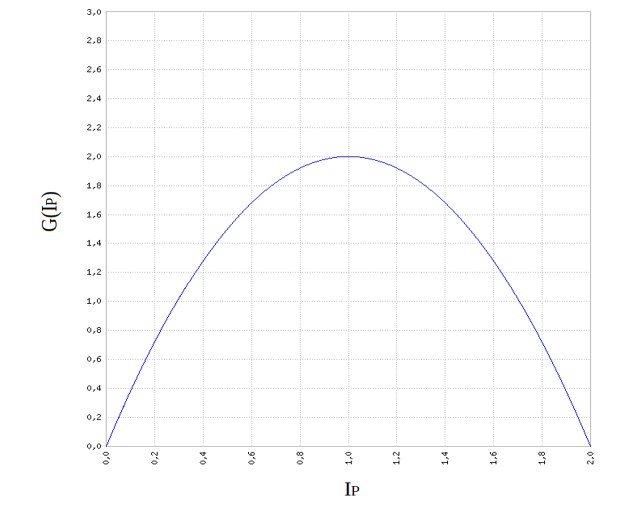
\includegraphics[width=1.0\textwidth]{figures/Prod-I.jpg}\end{figure}

Le terme de friction quadratique entraîne qu'au delà d'un certain seuil
$(I_{P}=\Delta\Pi/2R_{P})$, augmenter encore l'intensité de production diminue
en fait le flux extrait $G$.

Lorsque l'on souhaite atteindre un certain niveau de flux d'extraction G, il y
a donc zéro, une, ou deux intensités de production possible. S'il y en a deux,
on choisira systématiquement la plus basse. Ainsi, la valeur $(I_{P}=\Delta
\Pi/2R_{P})$, qui permet d'atteindre le flux d'extraction maximal est aussi la
valeur maximale de $I_{P}$. On notera cette valeur $I_{p}^{max}$.

De plus, il est possible que le niveau de flux d'extraction G requis ne soit
pas atteignable, selon le couple $(\Delta\Pi,R_{P})$. La valeur maximale de G
est
\[
G^{max}=\Delta\Pi^{2}/4R_{P}%
\]


Il est donc possible que la sphère économique fixe une requête de
production qui ne puisse pas etre satisfaite. La possibilité de ce
\textit{défaut de production} constitue le coeur du modèle: c'est là
que se manifeste la rétroaction de la sphère physique sur l'activité
économique. Un tel défaut de production est favorisé par~:

\begin{itemize}
\item Une requête de production élevée

\item Une différence de potentiel faible (on parle de \textit{pincement des
potentiels})

\item Une résistance élevée
\end{itemize}

De plus, l'efficacité du processus d'extraction, définie par $\eta=G/F_{HP}$,
vaut:\ \ \ \ \ \ \ \ \ \ \ \ \ \ \ \ \ \ \ \
\[
\eta=1-\Pi_{L}/\Pi_{H}-R_{P}I_{P}^{2}/F_{HP}%
\]


A intensité nulle, on retrouve une expression analogue au rendement de Carnot.
Ensuite, l'efficacité diminue a mesure que l'intensité augmente. Il s'agit
donc de trouver un compromis entre efficacité $\eta$ et flux extrait $G$.
Enfin, le processus d'extraction possède une certaine inertie. Si l'on est
capable instantanément de calculer l'intensité de production idéale permettant
de répondre a la requête de la sphère économique, l'intensité de
production réelle s'ajuste avec un certain retard. On définit une
\textit{intensité de production demandée }$I_{P}^{D}$. Le retard est
caractérisé par un \textit{temps caractéristique de réponse de production
}$\tau$.

On a alors~:\ \ \ \ \ \ \ $\ \ \ \ \ \ \ \ \ \ \ \ \ $%
\[
dI_{P}/dt+\tau I_{P}=I_{P}^{D}%
\]


Remarquons que cela permet de donner une signification physique au temps du
modèle. Désormais, la période de $t=10$ à $t=20$ dans le modèles,
soit $\Delta t=10$, peut etre comparé aux temps de réaction des feuilles, qui
eux ont une signification physique.

\subsection{Zone de recyclage}

Le flux de recyclage naturel est donné par la relation:

%

\[
F_{NR}=r\left(  1-\exp\left(  \frac{X_{L}}{0.5X_{T}}\right)  \right)
\]


ou r le taux de régénération naturel.

Parfois, un processus permettant de recycler une ressource est connu et
maîtrisé par l'Homme. On parle de recyclage "~humain~", par opposition au
recyclage naturel. Ces processus de recyclage humain sont des activités
économiques à part entière, et le recyclage d'une unité de ressource
nécessite un apport d'énergie (et de matière). Dans l'état actuel du
modèle, on suppose que recycler "~humainement~" une unité de ressource
nécessite un apport de \textit{x} unités d'énergie. La valeur \textit{x
}correspond au paramètre \textbf{recyclingEnergy}, spécifique a chaque
feuillet\footnote{Remarquons que ce choix de modélisation est peu réaliste.
Non seulement il faut en général d'autres ressources que juste de l'énergie
pour opérer un processus de recyclage, mais la difficulté a recycler (c'est a
dire la quantité d'énergie a apporter pour recycler une unité de ressource)
varie, selon la qualité du déchet. Ce point sera a améliorer dans la suite du
développement du modèle.}. On a introduit ici une notion de finalité de la
production~: la combinaison de certaines ressources permet de produire un bien
(ici un service)~: le recyclage d'une autre ressource. Les notions de
\textit{\ bien final} et de \textit{recettes de production} formalisent cette
idée. Dans le modèle, elles sont implémentées au niveau de la sphère
physique, au-dessus des différentes feuilles ressources. On parle de noyau
central, englobant toutes les feuilles ressources.

\section{Annexe C: Equations gouvernants un feuillet flux}

Un feuillet de type "~flux~" est défini par un flux incident $P_{i}$ (intégré
sur toute la surface de la Terre), et un appareil de production caractérisé
par un rendement $\eta$ et une surface installée $S$ (en pourcentage de la
surface terrestre). L'appareil de production permet l'extraction de cette
ressource, c'est a dire sa mise à disposition pour une transformation ultérieure.

Le flux extrait est~:$\ \ \ \ \ \ \ \ \ \ \ \ \ \ \ \ \ \ \ \ $%
\[
G=\eta P_{i}S
\]


Ce flux peut etre immédiatement utilisé, ou stocké en attente d'utilisation.
La capacité de stockage est définie par le paramètre $stock_{Max}$.

L'utilisation de la ressource correspond à un flux sortant du stock, noté
$G_{USED}$.

Ainsi, le stock $X_{S}$ vérifie~:\ \ \ \ \ \ \ \ \ \ \ \ \ \ \ \ \ \ \ \
\begin{align*}
\Delta X_{S}  &  =G-G_{USED}\\
0  &  <X_{S}<stock_{Max}%
\end{align*}
\ \ \ \ 

\section{Annexe D: Gestion du noyau central couplant les feuillets physiques:
"recettes"}

Le noyau central est la zone d'assemblage des ressources précédemment
extraites pour formation des biens finaux. Les recettes de production
définissent les ingrédients et quantités nécessaire a la formation d'une unité
d'un bien final. Par exemple, on peut définir le bien final "~barque~" avec la recette~:

\ \ \ \ \ \ \ \ \ \ \ \ \ \ \ \ 5 bois + 3 énergie = 1 barque

L'ensemble des coefficients des recettes définit une \textit{matrice des
recettes}, dont les colonnes représentent les ressources et les lignes les
biens finaux.

On suppose que les requêtes de la sphère économique s'expriment en unité
de bien final. Les requêtes de production de chaque ressource se déduisent
grâce aux coefficients des recettes.

Comme les recettes définissent des proportions entre les ressources, les
productions de chaque ressources doivent s'ajuster les unes aux autres en
permanence. Par exemple, en reprenant l'exemple précédent, si la production de
bois chute, la production d'énergie doit diminuer d'autant~: il ne sert à
rien de continuer à bruler du pétrole si l'on n'utilise pas l'énergie produite.

La mise en place de stratégies permettant d'obtenir ce résultat a fait l'objet
de plusieurs tentatives\footnote{Dans une première tentative, le noyau central
indique (a chaque nouveau pas de temps) à chaque feuille le niveau de
production souhaité. Le noyau central doit donc recueillir depuis les feuilles
les informations concernant les quantités de ressources disponible pour
utilisation $(X_{S})$, les traiter, puis renvoyer a chaque feuille le niveau
de production requis pour l'instant suivant. La complexité de ce processus
augmente exponentiellement avec le nombre de ressources et le nombre de
recettes. Finalement, il a été impossible de réaliser un algorithme
satisfaisant permettant de traiter toutes ces données, car un tel algorithme
nécessite l'introduction de multiples tests conditionnels qui rendent le
processus tres peu stable. Remarquons enfin que ce fonctionnement est peu
naturel (dans un systeme de marchés), puisqu'il correspond a l'hypothèse d'une
entité centrale régulatrice qui indique a chaque secteur de production le
niveau de production requis en fonction des résultats des autres secteurs.}.

Dans la stratégie retenue on fixe à chaque feuillet un objectif de stock
à atteindre. Ensuite, l'intensité de production de chaque feuille s'ajuste
afin de faire converger la valeur du stock vers le stock cible, et de l'y
maintenir. Plus précisément, la variation de l'intensité de production
demandée $\Delta I_{P}^{D}$ est donnée par
l'équation~:$\ \ \ \ \ \ \ \ \ \ \ \ \ \ \ \ $%
\[
\Delta I_{P}^{D}=a(X_{S}-X_{S}^{CIBLE})+b(dX_{S}/dt-0)
\]


On souhaite que $X_{S}$converge vers $X_{S}^{CIBLE}$, et $dX_{S}/dt$ vers 0~:
$\Delta I_{P}^{D}$ est donc fonction des écarts $X_{S}-X_{S}^{CIBLE}$ et
$dX_{S}/dt-0$. A l'équilibre, $\Delta I_{P}^{D}$est nulle.

$a$ et $b$ sont des paramètres définissant la préférence relative entre
les deux objectifs ($X_{S}=X_{S}^{CIBLE}$ et $dX_{S}/dt=0$).

\begin{figure}[h]
\centering
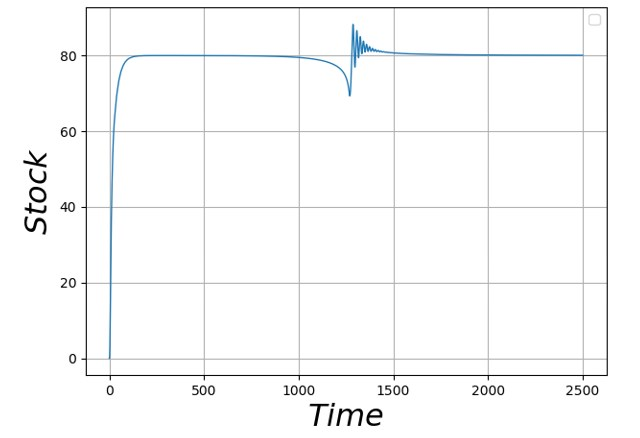
\includegraphics[width=1.0\textwidth]{figures/Stock-t.jpg}\end{figure}

Dans cette stratégie, chaque feuillet fixe de manière autonome son
intensité de production. On décrit ainsi une situation o{u} chaque secteur
de production auto-régule sa production en fonction de ce qu'il vend.
L'introduction de la notion de recette permet également de faire apparaître
l'idée qu'on ne peut pas produire de bien final sans énergie. En effet, la
recette de production indique la quantité d'énergie nécessaire à la
réalisation d'une unité de bien final. Si cette quantité n'est pas disponible,
on ne produit pas de bien final, c'est à dire qu'on "~n'utilise~" pas la
ressource qui a été extraite pour, une fois associée à de l'énergie, être
transformée en un bien final. Face à cette non utilisation, et afin de ne
pas constituer de stock trop important, la feuille ressource va de manière
autonome diminuer son intensité de production. Ainsi, l'introduction de la
notion de recette permet de rétroagir sur l'extraction de toutes les
ressources en cas de manque d'énergie~: on ne peut rien produire sans énergie.
Ce raisonnement est également valable en cas de défaut de production d'une
ressource autre qu'énergétique.

Ainsi, chaque feuille extrait à chaque pas de temps une certaine quantité
de ressources. Elle s'ajoute à la quantité de ressources "en stock"
$X_{S}$ disponible pour transformation ultérieure. La détermination du nombre
d'unités de biens finaux produits est fonction:

\begin{itemize}
\item des quantités de ressources ``en stock''

\item des requêtes de production de bien final provenant de la sphère économique

\item de la matrice des recettes~
\end{itemize}

Il s'agit donc d'allouer les ressources aux différentes recettes de production
de biens finaux. Il existe différentes méthodes d'allocations possibles. Par
exemple~: prioriser absolument la production du bien final $n^{o}1$ au
détriment de tous les autres, ou, a l'inverse, produire des biens finaux en
quantité égale sans tenir compte des requêtes de production, ou encore,
produire des biens finaux en respectant au maximum les proportions définies
par les requêtes de production émanant de la sphère économique.

Cette derniere stratégie semble la plus naturelle. Cela signifie que l'on
considère que les requêtes de production de biens finaux correspondent
à la demande du marché, et que l'on souhaiterait satisfaire toutes les
demandes simultanément, mais qu'en cas d'impossibilité, on répartit le défaut
de production entre tous les biens finaux utilisant cette ressources.
L'algorithme renvoie les allocations des ressources à la production des
différents biens finaux.

\subsection{Mix énergétique}

Lorsque la production d'un bien requiert de l'énergie, elle peut être réalisée
quelle que soit la provenance de cette énergie: pétrole, charbon, gaz,
nucléaire, solaire, etc. Il faut donc spécifier dans la recette le besoin en
énergie, et non pas le besoin en chaque ressource énergétique. Cela implique
qu'il faut indiquer, parmi les feuilles, lesquelles sont des ressources
énergétiques. On utilise ensuite ces ressources pour répondre au besoin en
énergie. On définit ainsi un mix énergétique effectif.

De plus, on définit lors du lancement d'une simulation un mix énergétique
souhaité, que l'on va chercher a satisfaire lorsque c'est possible. Le mix
énergétique effectif peut etre différent du mix énergétique souhaité, par
exemple si une ressource énergétique vient a manquer.

Finalement, la sphère physique décrit l'évolution de l'état de la
ressource au cours du temps, et comptabilise les flux de matiere et d'énergie
engendrés par la production de biens et par le recyclage. Mais les niveaux de
production et de recyclage souhaités sont des décisions humaines, auxquels la
sphère physique ne fait que répondre. Les lois décrivant l'évolution de
ces requêtes sont décrites dans la sphère économique.

\section{\textbf{{Annexe E: Economie}}}

\subsection{{S}phère économique}

\subsubsection{{Structure générale}}

Le rôle de la sphère économique est de spécifier l'évolution de l'ensemble
des variables économiques. En particulier, elle indique a la sphère physique~:

\begin{itemize}
\item des requêtes de production pour chaque bien final

\item une requête de recyclage ``humain'' pour chaque ressource concernée

\item le mix énergétique souhaité

\item l'investissement, pour chaque secteur (feuille), qui permet d'augmenter
le capital. Le capital est directement relié a la résistance R$_{P}$des
feuilles ``stock'', et aux variables \textit{surface installée} S et stockMax
des feuilles ``flux''

\item le niveau de stock cible pour les feuilles de type ``stock''
\end{itemize}

\subsubsection{{progrès technique}}

On spécifie dans la sphère économique les lois décrivant le progrès
technique éventuel. Le progrès technique correspond ici a la diminution
des quantités de ressources nécessaires à la production d'une unité de
bien final. C'est donc un gain d'efficacité: il faut moins d'énergie pour
usiner une pièce, ou moins d'aluminium pour produire une canette. Dans le
modèle, cela correspond à la diminution des coefficients de la matrice
des recettes. La découverte d'un nouveau matériau, ou le développement d'une
technologie permettant de substituer un matériau par un autre constitue une
autre forme de progrès technologique.\footnote{Par exemple, dans les années
1970, la demande en nickel a chuté de 20\%, principalement a cause de la
substitution du manganese au nickel dans la production de pare-chocs
automobiles\cite{Godard1980}.} Dans la suite du développement du modèle,
la notion de substitution pourra etre représentée par une modification des
recettes de production. Remarquons bien que la sphère économique n'adresse
que des "requêtes de production" à la sphère physique. Cela implique
que ces requêtes peuvent être, ou non, satisfaite, par exemple en cas de
pincement des potentiels décrivant l'état de la ressource. Ce point est
capital, puisqu' il implique la possibilité d' une rétroaction de la
sphère physique sur la sphère économique. L' ensemble de lois
décrivant l'évolution de ces variables constitue la sphère économique. L'
architecture du code du modèles rends ces lois accessibles et modifiables
facilement. Dans la démarche du projet, l' utilisateur est encouragé à
tester divers paramètres, lois et modèles macroéconomiques. Une
bibliothèque d' exemples de telles lois commence à être constituée. En
particulier, on peut utiliser comme requête de production les fonctions de
production de modèles macroéconomiques, et comme investissement celui
décrit par ces mêmes modèles.

\subsubsection{\ Niveaux d'utilisation du modèle}

Il existe plusieurs niveaux d' utilisation du modèle:

\begin{enumerate}
\item le premier niveau consiste a faire tourner le modèle en utilisant
dans la sphère économiques des lois déjà pré-écrites et en faisant
uniquement varier les paramètres (nombre de ressources, leurs
caractéristiques, choix du mix énergétique, recyclage demandé, etc). Par
exemple, a faire varier le taux de croissance de la productivité du travail
dans un modèle de Solow.

\item Le second niveau consiste a tester diverses lois (et modèles
macro-économiques) parmi la bibliothèque de lois disponibles. Cela permet
d' observer la sensibilité de la sphère physique au choix de ces lois.

\item Enfin, l' utilisateur maîtrisant déjà bien le modèle est invité
a proposer de nouvelles lois lui-même, afin d' enrichir la bibliotheque. Une
loi peut correspondre par exemple a la fonction de production d' un modèle
macroéconomique, a une hypothese concernant le rythme du progres technique, ou
a l' introduction d' une rétroaction entre l'état des ressources et le mix
énergétique souhaité.
\end{enumerate}

\subsubsection{{Exemple de modèle: Solow}}

{Un exemple de sphère économique basée sur le modèle de Solow}

\begin{figure}[h]
\centering 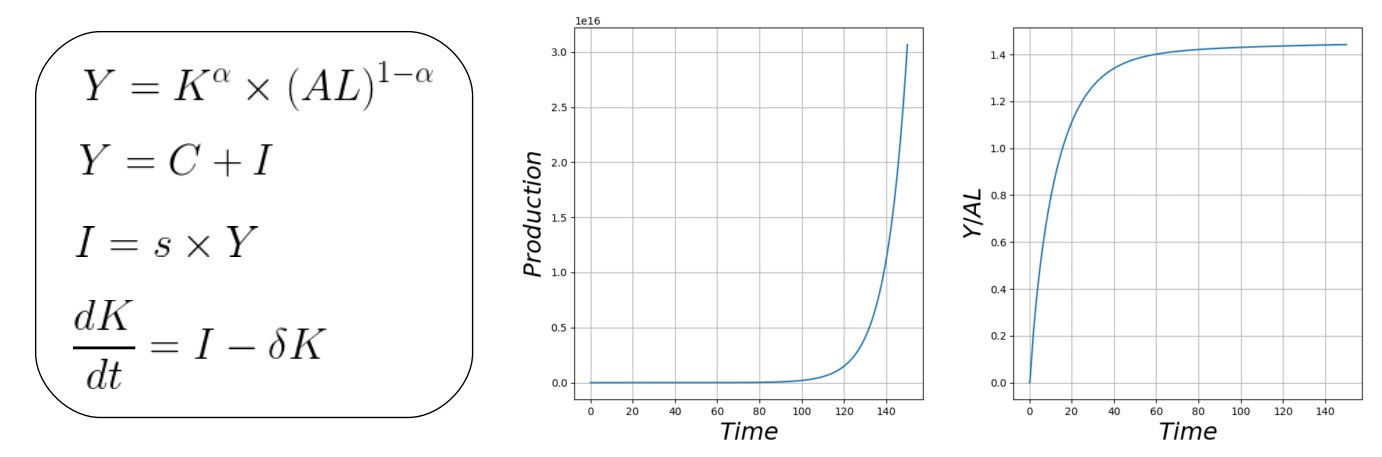
\includegraphics[width=1.0\textwidth]{figures/solow2.jpg}\end{figure}

Le modèle de Solow, créé en 1956, est un modèle macroéconomique qui
explique la croissance par l' accumulation du capital, la croissance de la
population active, et la croissance de la productivité du travail. C' est un
modèle de référence de l'économie néo-classique.

Il utilise une fonction de production de Cobb-Douglas a deux facteurs :%

\[
Y=K^{\alpha}(AL)^{1-\alpha}%
\]


avec :

\begin{itemize}
\item $Y$ la production

\item $K$ le capital

\item $A$ la productivité du travail

\item $L$ la population active
\end{itemize}

La productivité du travail augmente de maniere exogene, au taux g$_{A }$.

La population active augmente également de maniere exogene. Dans notre
modèle, on choisit de faire tendre la population active vers une valeur
limite P$_{L}$: le taux de croissance de la population active est
$g_{L}=q(1-L/P_{L})$. Le taux de croissance diminue a mesure que la population
active L se rapproche de sa valeur limite P$_{L}$.

Le capital s'érode au taux $\delta K$, érosion compensée par l' investissement I.

\ \ \ \ \ \ \ \ \ \ \ \
\[
\frac{dK}{dt} = I-\delta K
\]


Une part \textit{s} de la production est réinvestie :

\ \ \ \ \ \ \ \ \ \ \
\[
\ I=sY\ \
\]
\ \ 

Dans ce modèle, la production Y augmente exponentiellement, grâce a la
croissance de la productivité du travail. La production par unité de travail
effectif Y/AL converge vers un état stationnaire.

\subsection{Adaptation pour la sphère économique}

\subsubsection{Fonction de requête de production}

On utilise la fonction de production du modèle de Solow comme fonction de
requête de production (section 1.2.1).

On initialise les requêtes de production de chaque bien final au lancement de
la simulation. A chaque instant, on calcule la requête pour l'instant t+dt
à partir du résultat de production de l'instant t%

\[
Y_{REQ}(t+dt)=Y(t)\ast\left(  \frac{K(t+dt)}{K(t)}\right)  ^{\alpha}\left(
\frac{A(t+dt)L(t+dt)}{A(t)L(t)}\right)  ^{1-\alpha}%
\]
\ \ avec

\begin{itemize}
\item $Y_{REQ}$ la requête de production adressée a la sphère physique.

\item $Y$ la production effective (qui peut différer de la requête de production)
\end{itemize}

Ainsi, tant que la requête de production est satisfaite, la production est
égale à celle prédite par le modèle de Solow. Si la requête de
production n'est pas satisfaite à l'instant t, la requête à l'instant
t+dt s'adapte : on ne continue pas à demander une croissance exponentielle
indéfiniment alors que la production effective ne suit plus.

\subsubsection{Investissement}

L'investissement est défini pour chaque feuille ressource. On définit un
paramètre s commun à toutes les feuilles, qui correspond à la
fraction de la production réinvestie. La production de chaque feuille
correspond à ce qui a été effectivement utilisé par le noyau central de le
sphère physique, c'est à dire la variable $G_{USED}$.

Ainsi,

\qquad\qquad\qquad\qquad\qquad\qquad%
\[
I=sG_{USED}%
\]


\subsubsection{Requête de recyclage}

Pour la requête de recyclage, on définit la loi suivante : on souhaite
recycler une proportion constante de la quantité de déchets produits On
définit cette proportion à l'initialisation de la simulation., en
indiquant la valeur du paramètre recycling compris entre 0 et 1.

L'équation de la requête de recyclage est donc :%

\[
Y_{REQ}(t+dt)=(F_{LP}(t)+G_{USED}(t))\ast recycling
\]


Cette loi n'est qu'une proposition. On pourrait également tenir compte de la
quantité totale de déchets $X_{L}$ pour la requête de recyclage, et non pas
simplement de la variation de cette quantité.

\subsubsection{Autres inputs économiques}

Il a été choisi de ne pas faire varier le niveau cible de stock demandé aux
feuillets, ni le mix énergétique souhaité, ni les quantités de ressources
nécessaires à la production d'une unité de chaque bien final (coefficients
de la matrice des recettes). Le modèle a été créé dans un souci de
permettre à l'utilisateur de proposer et tester ses propres fonctions et
scénarios de variation de toutes ces requêtes de la sphère économique
à la sphère physique. Ainsi, la partie contenant toutes les fonctions
accessibles à l'utilisateur est située dans un fichier à part, court
et commenté.

\subsection{Analyse}

Ce modèle n'a pas pour but de reproduire le plus fidèlement possible
la trajectoire de l'économie mondiale des dernières décennies, ni de
prédire quantitativement ce qui pourrait advenir. Il s'agit d'un outil
permettant de tester une multitude d'hypothèses, de scénarios, de
modèles macro-économiques dans un cadre prenant en compte explicitement
l'impact de l'activité économique sur la sphère physique et les
rétroactions de celle-ci.

Le nombre d'hypothèses et scénarios pouvant être testés n'est limité que
par l'imagination de l'utilisateur. Par conséquent, cette partie n'a pas pour
ambition de livrer une analyse complète de ce que l'on peut tirer du
modèle, mais de livrer quelques résultats fondamentaux obtenus. On tachera
de présenter ces résultats, puis de les illustrer au moyen d'un exemple qui
permet d'isoler le phénomène ou motif discuté.

On retrouve des résultats attendus, mais qui ne sont pas obtenus par la
plupart des modèles macroéconomiques. Cela permet de vérifier que cet
outil atteint son objectif de proposer une base physique aux modèles
macroéconomiques via la prise en compte directe des flux de matière et
d'énergie engendrés par l'activité économique.

\section{Annexe F: Mécanisme de rétroaction Physique-Economique}

\subsection{Rétroactions de la sphère physique sur l'activité économique}

On observe, selon le paramétrage de la situation, des rétroactions de la
sphère physique sur l'activité économique. En particulier, lorsque le flux
de recyclage (naturel ou humain) est nul (ressources non recyclables par
exemple) ou insuffisant, on observe l'épuisement des ressources "`stock"', et
leur rétroaction sur la production. Cette rétroaction prend la forme de
rupture de pentes : il s'agit donc d'effondrement davantage que de diminution
progressive. Illustrons ce point par un exemple jouet qui permet de faire
apparaître le mécanisme de l'effondrement.

On considère un monde à trois ressources, cuivre, bois et pétrole. Ces
trois ressources permettent de produire deux biens finaux, selon les recettes :

\textbullet\qquad cuivre + énergie = bien 0

\textbullet\qquad cuivre + bois + énergie = bien 1

Par souci de simplicité, on considère que l'on n'est pas capable de
recycler le cuivre (ou que l'on ne le souhaite pas). Le bois se recycle
naturellement. On suppose également que les résistances des appareils de
production sont constantes (érosion du capital et investissement nuls)

Enfin, on se place dans un scénario de croissance nulle. La demande en biens
finaux est constante (respectivement 12 bien 0 et 18 bien 1 par unité de temps).

\begin{figure}[h]
\centering
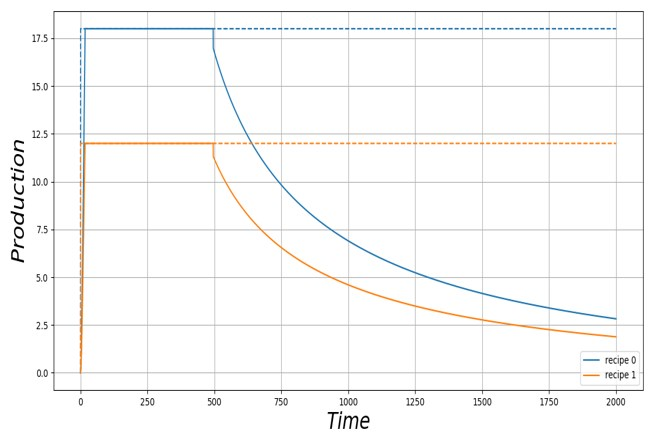
\includegraphics[width=1.0\textwidth]{figures/Production7.jpg}\end{figure}

On observe une chute de la production des biens 1 et 2 à t=500, malgré une
requête de production constante. La production semble converger
exponentiellement vers une production nulle (ce qui est confirmé par un
passage en échelle logarithmique).

Les ressources cuivre et pétrole (seule ressource énergétique de la
simulation) sont communes aux deux recettes de production. La simultanéité des
chutes de production des biens 0 et 1 suggère que l'une de ces deux
ressources à fait défaut.

\begin{figure}[h]\centering  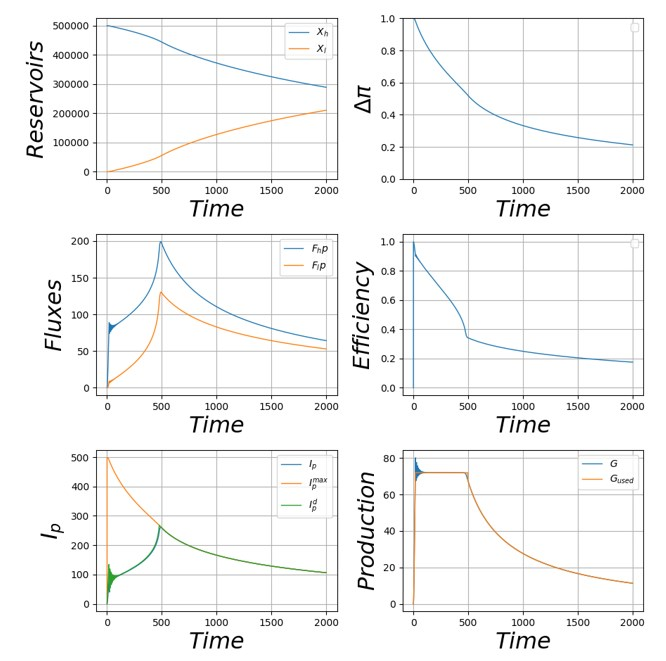
\includegraphics[width=1.0\textwidth]{figures/Tableau-Bord8.jpg}\end{figure}

En effet, l'état de la ressource pétrole semble s'être dégradé rapidement,
entraînant une chute de la production de pétrole à t=500. Examinons le
mécanisme menant à cet effondrement.

La figure 8a indique que le réservoir haut se vide progressivement, tandis que
le réservoir bas se remplit. En conséquence, la différence de potentiels
diminue (figure 8b). Malgré une requête de production constante, les flux de
pétrole venant du réservoir haut (FHP) et en direction du réservoir bas (FLP)
augmentent rapidement, à cause du pincement des potentiels (figure 8c).
Dans le même temps, l'efficacité du processus chute (figure 8d). L'intensité
de production augmente pour compenser la chute de l'efficacité et satisfaire
la requête. L'intensité de production maximale possible diminue, et à
t=500, l'intensité de production atteint l'intensité de production maximale
(figure 8e). Immédiatement, la production chute (figure 8f).

Ainsi, un scénario de croissance nulle, sans recyclage, entraîne un
emballement avec une explosion des flux de ressource afin de compenser la
perte d'efficacité, dans un cercle vicieux. On observe ici un défaut de
production lié à l'épuisement d'une ressource non-renouvelable et non-substituée.

\subsection{Etat stable}

Cependant, une activité économique stable (qui ne s'effondre pas à temps
infini) est possible, si elle n'implique l'utilisation que de ressources stock
recyclables (naturellement ou humainement) et de ressources renouvelables
(ressources flux).

Pour illustrer ce point, on se place dans une situation similaire à
l'exemple précédent, en remplaçant la feuille "`pétrole"' par une feuille
"`énergie solaire"'. La demande en biens finaux 0 et 1 est constante. On
suppose que la ressource bois est très abondante, contrairement à la
ressource cuivre. Cependant, on est capable de recycler le cuivre, au moyen
d'un apport d'énergie : une unité d'énergie permet de recycler une unité de cuivre.

On suppose également que la surface de panneaux solaires installée est
très importante, et qu'il n'y a pas d'érosion du capital. Ainsi, la
quantité d'énergie renouvelable est largement supérieure aux besoins de
l'activité économique. C'est une hypothèse forte.

De $t=0$ à $t=500$, on décide de ne pas recycler le cuivre. $At=500$ et
pour tous les instants ultérieurs, on décide de recycler 100 \% des déchets de
cuivre nouvellement produit.

Le système semble stable (Fig. \ref{Fig9}). Mais l'observation de
l'évolution de l'état de la ressource cuivre montre que la décision de fixer
une requête de recyclage de 100 \% à t=500 à permis d'éviter un
effondrement, et d'atteindre cet état stable (Fig. \ref{Fig10}).

\begin{figure}[h]
\centering
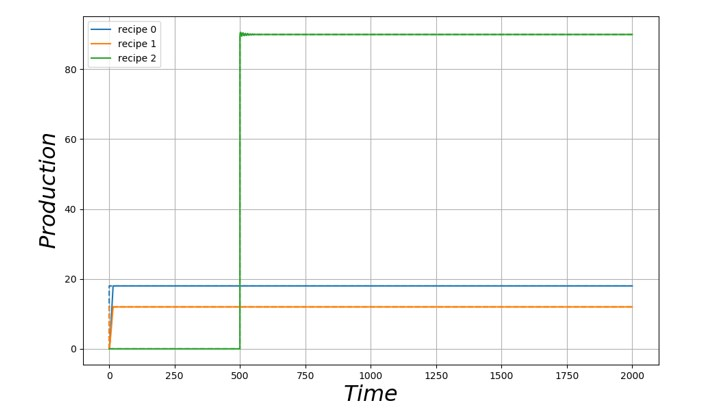
\includegraphics[width=1.0\textwidth]{figures/Production9.jpg}\label{Fig9}\end{figure}

\begin{figure}[h]
\centering
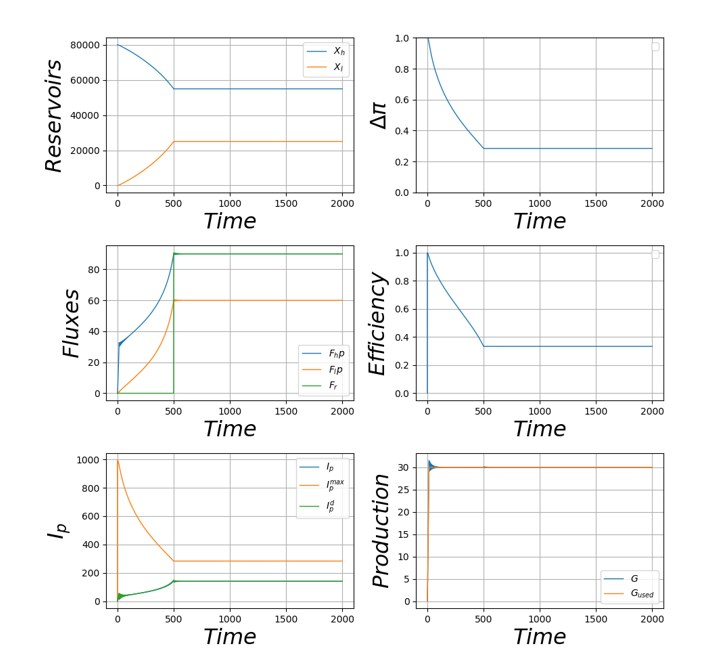
\includegraphics[width=1.0\textwidth]{figures/Tableau-Bord10.jpg}\label{Fig10}\end{figure}

\subsection{Passage d'une économie basée sur des ressources flux à une
économie basée sur des ressources stock}

Il existe donc, pour un ensemble de ressources et de recettes donnée, un
niveau de production stable maximum. L'activité économique peut dépasser ce
niveau stable maximum grâce à l'usage de ressources "`stock"' dont le
rythme d'exploitation est virtuellement illimité. Mais si l'exploitation de
ces ressources est plus rapide que le recyclage naturel, ou si elle ne
s'accompagne pas d'une augmentation égale du recyclage humain (en particulier
si celui-ci est impossible, comme pour les ressources fossiles), on risque de
dégrader ces ressources, si bien que le nouvel état n'est pas stable.

En fin de compte, les facteurs limitant sont :

\textbullet\qquad l'utilisation de ressources stock que l'on ne sait pas
recycler, et pour lesquelles on ne trouve pas de substituts.

\textbullet\qquad La production d'énergie renouvelable, nécessaire au
recyclage de toutes les autres ressources stock.

Si les ressources stock s'épuisent, on revient de manière forcé à un
niveau stable, vérifiant les conditions énoncées précédemment (section 2.2).
La dégradation de l'état des ressources stock advenue est irréversible, et le
nouveau niveau de production stable maximum a diminué.

Afin d'illustrer ces propos, on considère un monde à quatre ressources
: cuivre, bois, pétrole et énergie solaire. Par souci de simplicité, on
suppose à nouveau que l'on ne sait pas recycler le cuivre, mais que cette
ressource est extrêmement abondante. On suppose également que le taux de
régénération du bois est très élevé.

On considère les mêmes recettes que précédemment (section 2.1). La requête
de production des biens finaux suit une trajectoire de croissance
exponentielle obtenue par une loi de type "`Solow"' , semblable à celle
décrite en section 1.2.2.2. Les requêtes de production initiales sont proches
de zéro.

Le mix énergétique souhaité est : 100 \% d'énergie solaire. Le mix énergétique
réel peut être différent, si le mix énergétique souhaité ne permet pas de
répondre aux requêtes de production.

\begin{figure}[h]
\centering
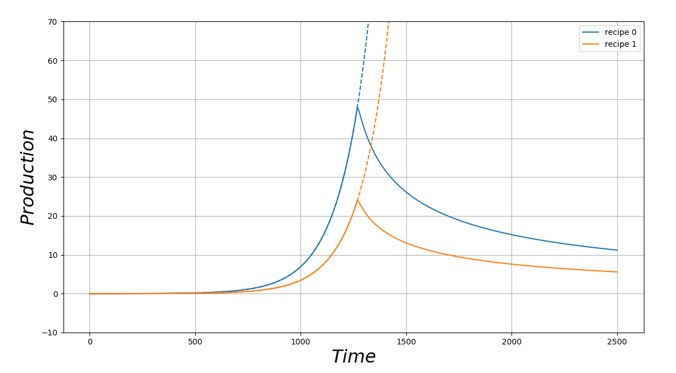
\includegraphics[width=1.0\textwidth]{figures/Production11.jpg}\label{Fig11}\end{figure}

On observe (Fig. \ref{Fig11}) dans un premier temps une augmentation
exponentielle de la production de biens 1 et 2, suivant la croissance
exponentielle des requêtes de production. A t=1250, la production de biens 1
et 2 chute, et les requêtes de production ne sont plus satisfaites. Les flux
de production semblent converger vers un niveau plus faible mais non-nul.

\begin{figure}[h]
\centering
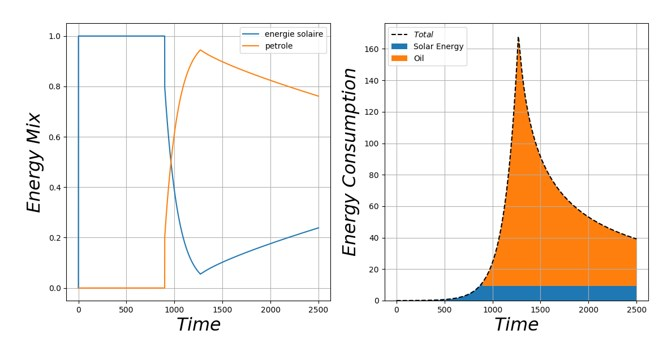
\includegraphics[width=1.0\textwidth]{figures/Energie12.jpg}\label{Fig12}\end{figure}

L'étude de l'évolution du mix énergétique réel au cours du temps indique que
dans un premier temps (t%
%TCIMACRO{\TEXTsymbol{<}}%
%BeginExpansion
$<$%
%EndExpansion
800), le besoin en énergie est entièrement couvert par la feuille
"`énergie solaire"' (Fig. \ref{Fig12}). Le mix énergétique réel est donc égal
au mix énergétique souhaité. Pour t%
%TCIMACRO{\TEXTsymbol{>}}%
%BeginExpansion
$>$%
%EndExpansion
800, le besoin en énergie dépasse la production d'énergie solaire. On fait
donc appel à la feuille pétrole afin de continuer à satisfaire la
requête en énergie. Le mix énergétique réel voit la place du pétrole devenir
prépondérante, à mesure que la demande en énergie croit. La feuille
pétrole permet donc de continuer à suivre la trajectoire de croissance
exponentielle au-delà du niveau permis par l'utilisation unique de
l'énergie solaire. A t=1250, la production de pétrole chute, ce qui semble
indiquer un défaut de production de la feuille. Un regard sur l'évolution de
l'état de la feuille pétrole le confirme. La production de biens finaux chute,
suivant la production de pétrole. Le mix énergétique revient peu à peu
vers un mix 100 \% solaire. Les niveaux de production convergent vers le
niveau maximal permis par le flux d'énergie solaire disponible.

\subsection{Variations du capital}

Toutes les illustrations jusqu'ici proviennent de simulations avec capital
fixé : le taux d'érosion du capital \U{3b4} était nul, et l'investissement
également. Ainsi, les résistances $R_{P}$ des feuilles stock et paramètres
"`surface installée "`des feuilles flux étaient constantes. L'introduction
d'un taux d'érosion et d'un investissement non-nul modifie les trajectoires observées.

Dans la suite, on suppose que l'investissement dans le capital d'une feuille
est une proportion fixe de la production de cette feuille : le secteur " vend
" x unités de ressource, et en réinvestit une proportion s. C'est la loi
d'investissement décrite en section 1.2.2.2. Notons que les résultats
présentés ci-après dépendent fortement de cette loi d'investissement. En
particulier, il serait judicieux d'écrire une loi modélisant une situation ou
le secteur A peut choisir d'investir une part de ses revenus dans le secteur B
si celui-ci est plus " rentable ". Toute la démarche du projet consiste à
laisser accessible à l'utilisateur la partie de modélisation économique
afin de lui permettre, par exemple, de tester une telle loi.

Les notions d'érosion du capital et d'investissement entraînent l'apparition
de cercles vertueux et de cercles vicieux dans un contexte de requête de
production croissante.

Tant que la production augmente, l'investissement augmente. Le capital
augmente donc également, et la résistance RP diminue. Le terme de friction
diminue donc, et la valeur maximal du flux produit GMAX augmente. La
production peut donc augmenter encore d'avantage, et ainsi de suite.

A l'inverse, si la production chute, l'investissement chute, donc le capital
également, et la résistance augmente, ce qui aggrave encore la chute de la production.

Pour illustrer ces propos, on considère un monde à trois ressources :
cuivre, bois, pétrole, et deux recettes (les mêmes que précédemment). Le
cuivre et le bois sont supposés très abondants. La requête de production
est exponentiellement croissante. On effectue deux simulations successives,
une avec érosion du capital et investissement nuls, une seconde avec érosion
du capital et investissement positifs (Fig. \ref{Fig13}).

\begin{figure}[h]
\centering
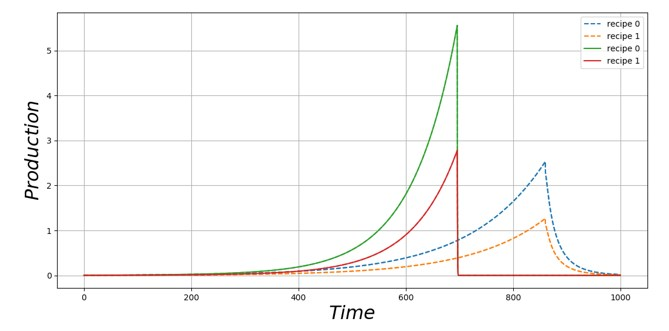
\includegraphics[width=1.0\textwidth]{figures/Production13.jpg}\label{Fig13}\end{figure}

On constate que la croissance et la décroissance sont bien plus rapide dans la
simulation avec investissement et érosion du capital. On peut l'expliquer en
examinant l'évolution de l'état de la feuille pétrole.

\begin{figure}[h]
\centering
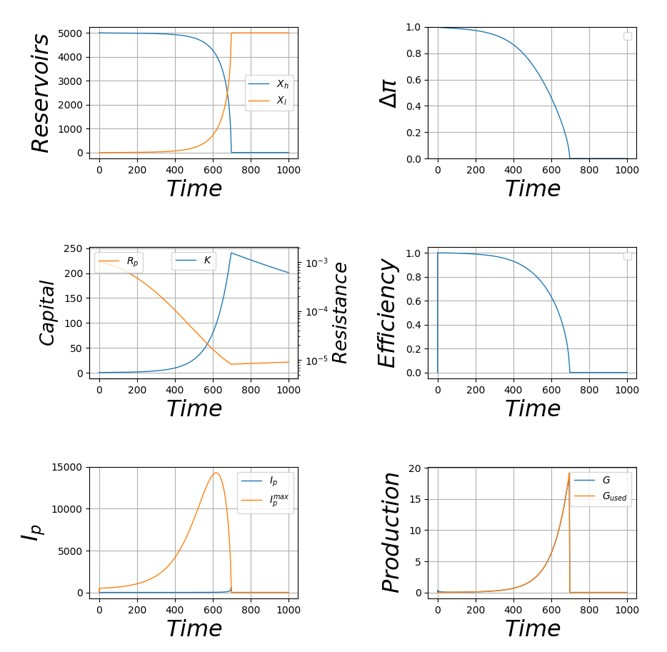
\includegraphics[width=1.0\textwidth]{figures/Tableau-Bord14.jpg}\label{Fig14}\end{figure}

De t=0 à t=700, la production de pétrole augmente, en réponse à
l'augmentation exponentielle des requêtes. L'investissement augmente donc, ce
qui permet d'augmenter le capital et de diminuer la résistance (Fig.
\ref{Fig14}c). Par conséquent, l'intensité de production maximale possible
augmente (Fig. \ref{Fig14}e). De plus, la diminution de la résistance compense
la chute de la différence de potentiel (Fig. \ref{Fig14}b). Ainsi, on parvient
à extraire presque toute la ressource du réservoir haut (Fig.
\ref{Fig14}a). A $t=700$, le réservoir haut est presque vide. Malgré la faible
valeur de la résistance, la production chute.

On rentre alors dans un cercle vicieux : l'investissement chute également, et
ne parvient plus à compenser l'érosion du capital. La résistance de
l'appareil de production augmente à nouveau, et la production ultérieure
est encore plus difficile. La chute s'accélère.

\section{Conclusion}

\begin{itemize}
\item Outil d'ancrage dans la réalité physique de n'importe quel modèle
macroéconomique, et observation de l'action de la sphère économique sur la
sphère physique.

\item modèle développé dans un souci de simplicité et modularité afin de
faciliter son appropriation par ses utilisateurs.

\item Modélisation du monde physique utilisant certaines catégories de la
thermodynamique sans revendication d'être un modèle thermodynamique.

\item requêtes économiques satisfaites ou non selon la disponibilité des
ressources physiques.
\end{itemize}

\begin{thebibliography}{99}                                                                                               %


\bibitem {Boulinding1966}Boulding, K.E. The economics of the coming spaceship
earth. In Environmental Quality in a Growing Economy.H. Jarrett, Ed.: 3--14.
Johns Hopkins University Press. Baltimore, 1966.

\bibitem {Roegen1971}Georgescu-Roegen, N. The Entropy Law and the Economic
Process. Harvard University Press. Cambridge, MA, 1971.

\bibitem {Sollner1997}Fritz Söllner, A reexamination of the role of
thermodynamics for environmental economics, Ecological Economics, Volume 22,
Issue 3, Pages 175-201, 1997.

\bibitem {Cutler1997}Cutler J Cleveland, Matthias Ruth, When, where, and by
how much do biophysical limits constrain the economic process?: A survey of
Nicholas Georgescu-Roegen's contribution to ecological economics, Ecological
Economics, Volume 22, Issue 3, Pages 203-223, 1997.

\bibitem {Daly1997a}Herman E Daly, Georgescu-Roegen versus Solow/Stiglitz,
Ecological Economics, Volume 22, Issue 3, Pages 261-266, 1997.

\bibitem {Solow1997}Robert M Solow, Georgescu-Roegen versus Solow-Stiglitz,
Ecological Economics, Volume 22, Issue 3, Pages 267-268, 1997.

\bibitem {Stiglitz1997}Joseph E Stiglitz, Georgescu-Roegen versus
Solow/Stiglitz, Ecological Economics, Volume 22, Issue 3, Pages 269-270, 1997.

\bibitem {Daly1997b}Herman E Daly, Reply to Solow/Stiglitz, Ecological
Economics, Volume 22, Issue 3, Pages 271-273, 1997,

\bibitem {Meadows1972}Meadows, D. H., Meadows, D.H., Randers, J\o rgen, et al.
The limits to growth: a report to the club of Rome (1972). 1972.

\bibitem {Glucina2010}Glucina, M. D. and Mayumi, K, Connecting thermodynamics
and economics. Annals of the New York Academy of Sciences, 1185: 11-29. (2010)

\bibitem {Godard1980}Godard O., Baillon J., Céron J., Substitutions et
économie sociale des ressources naturelles, page 15, 1980
\end{thebibliography}


\end{document}